\makeatletter\frontmatter@init\makeatother

\title{Radio-Frequency methods for Majorana-Based Quantum Devices: \\ Fast-Charge sensing and Phase-Diagram Mapping}

\author{D. Razmadze}
\author{D. Sabonis}
\author{F. K.~Malinowski}
\author{G. C. M\'enard}
\affiliation{Center for Quantum Devices, Niels Bohr Institute, University of Copenhagen and Microsoft Quantum Lab Copenhagen, Universitetsparken 5, 2100 Copenhagen, Denmark}
\author{S. J. Pauka}
\affiliation{Center for Quantum Devices, Niels Bohr Institute, University of Copenhagen and Microsoft Quantum Lab Copenhagen, Universitetsparken 5, 2100 Copenhagen, Denmark}
\affiliation{ARC Centre of Excellence for Engineered Quantum Systems, School of Physics, The University of Sydney,  NSW 2006, Sydney Australia}
\author{H. Nguyen}
\affiliation{Center for Quantum Devices, Niels Bohr Institute, University of Copenhagen and Microsoft Quantum Lab Copenhagen, Universitetsparken 5, 2100 Copenhagen, Denmark}
\affiliation{Nano and Energy Center, Hanoi University of Science, VNU 120401, Hanoi, Vietnam}
\author{D. M. T. van Zanten}
\author{E. C. T. O'Farrell}
\author{J. Suter}
\affiliation{Center for Quantum Devices, Niels Bohr Institute, University of Copenhagen and Microsoft Quantum Lab Copenhagen, Universitetsparken 5, 2100 Copenhagen, Denmark}
\author{P. Krogstrup}
\affiliation{Microsoft Quantum Materials Lab and Center for Quantum Devices, Niels Bohr Institute, University of Copenhagen, Kanalvej 7, 2800 Kongens Lyngby, Denmark}
\author{F. Kuemmeth}
\author{C. M. Marcus}
\affiliation{Center for Quantum Devices, Niels Bohr Institute, University of Copenhagen and Microsoft Quantum Lab Copenhagen, Universitetsparken 5, 2100 Copenhagen, Denmark}

\makeatletter
\begingroup
\@author@finish
\frontmatter@author@produce@script
\endgroup
\makeatother

\begin{abstract}
This section presents an extract from the above paper. Radio-frequency (rf) reflectometry is implemented in hybrid semiconductor-superconductor nanowire systems designed to probe Majorana zero modes. Nanowire devices are capacitively coupled to a nearby RF single-electron transistor made from a separate nanowire, allowing RF detection of charge, including charge-only measurement of the crossover from $2e$ inter-island charge transitions at zero magnetic field to $1e$ transitions at axial magnetic fields above \SI{0.6}{\tesla}, where a topological state is expected. Single-electron sensing yields signal-to-noise exceeding 3 and visibility $99.8\%$ for a measurement time of \SI{1}{\micro\second}.
\end{abstract}

\subsection{Introduction}

\begin{figure}
	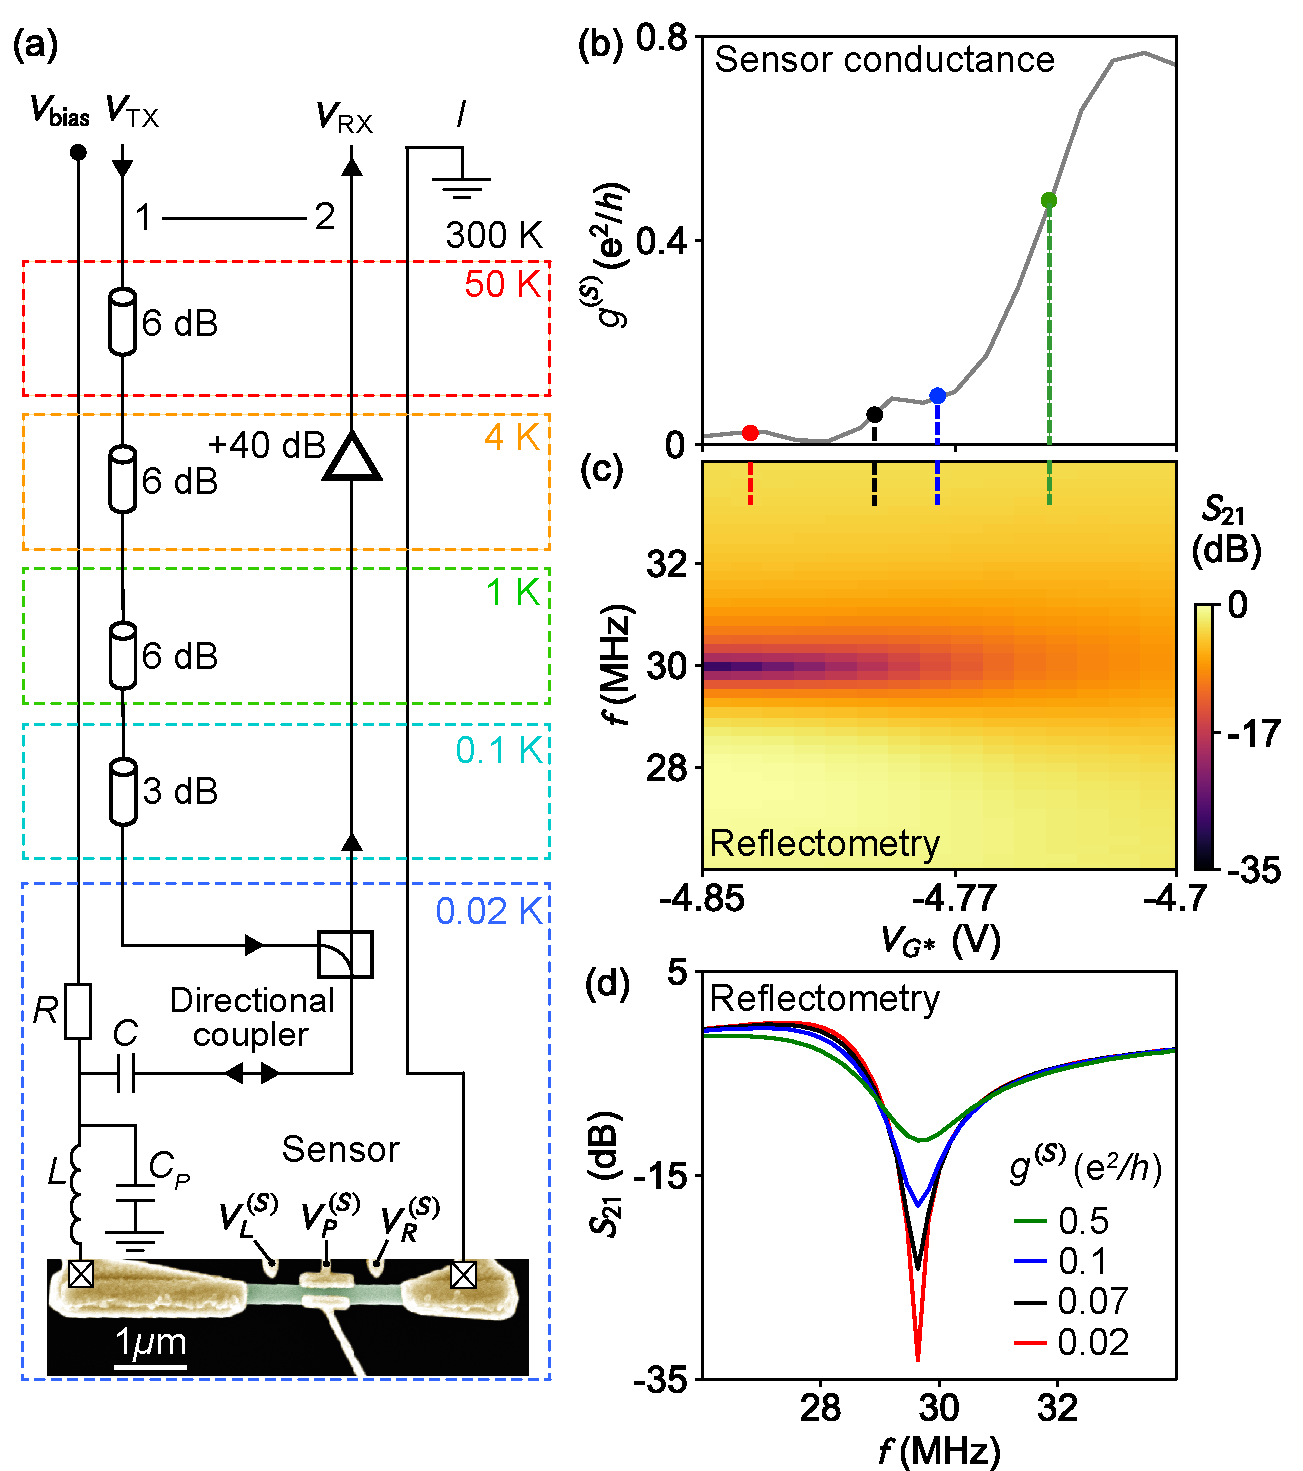
\includegraphics[width=0.65\textwidth]{Fig1-20.pdf}
	\caption[The rf charge-sensing setup]{(a) A circuit diagram of a nanowire (sensor) embedded in a resonant circuit allowing conductance by measuring current $I(V_\textrm{bias})$ or reflectometry measurement (by measuring reflected signal $V_\textrm{RX}$), respectively (see the main text). (b) The sensor conductance, $g^{(S)}$, as a function of the sensor gate voltage, $V_{G^{*}} = V_{L}^{(S)} = V_{P}^{(S)} = V_{R}^{(S)}$. (c) The scattering parameter, $S_{21}$, as a function of the carrier frequency $f$, and $V_{G^{*}}$ acquired simultaneously with (b). $S_{21}(f)$ develops a dip at $f_{\rm res}$ $\sim \SI{30}{\mega\hertz}$, indicating that the matching condition of the resonator is approached toward low sensor conductance. (d) Vertical cuts of (c) for the gate voltages indicated in (b). The on-resonance reflectometry signal acts as an alternative measure of $g^{(S)}$.}
	\label{fig:majo_a}
\end{figure}

Solid-state quantum computation schemes that involve repeated measurement and feedback, including topological schemes \cite{AasenPRX16, PhysRevB.94.235446, Plugge, PhysRevB.95.235305} with potentially long coherence times \cite{Non-Abelian, Alicea_2012}, nonetheless require fast read-out of charge or current in order to operate on reasonable time scales \cite{Reiher7555}. For topological qubits based on Majorana modes in nanowires (NWs) with proximity-induced superconductivity, quasiparticle poisoning of Majorana modes constrains read-out times to microseconds or faster \cite{Lossqpp}, as has already been demonstrated for superconducting \cite{SCq3,SCq2,SCq1,SCq4} and spin qubits \cite{Reilley1,sensingdot,petta,RevModPhys.79.1217}.

Here, we report the realization of radio-frequency (rf) reflectometry in various configurations of InAs nanowires (NWs) with epitaxial Al, fabricated to form single or coupled Majorana islands, with proximal NW charge sensors. The device geometries are inspired by recent theoretical proposals for demonstrating elementary topological qubit operations in these systems \cite{AasenPRX16, PhysRevB.94.235446, Plugge, PhysRevB.95.235305}. A resonator is capacitively coupled to a proximal NW charge sensor configured for both LF and rf charge read-out. The overall charge sensitivity is investigated as a function of the measurement time and is found to yield a signal-to-noise ratio (SNR) for single-charge detection exceeding 3 and a visibility of $99.8\%$ for an integration time of \SI{1}{\micro\second}, with correspondingly higher values for longer integration times. Proximal NW charge sensors are found to be compatible with magnetic fields exceeding \SI{1}{\tesla}, the range needed to reach the topological regime \cite{Mourik1003,MT1,nature26142,AlbretchNature}. All measurements are carried out in a dilution refrigerator (Oxford Instruments Triton 400) a base temperature of approximately \SI{20}{\mk}, equipped with a 6-1-1~\si{\tesla} vector magnet.

\subsection{Experimental setup}

The reflectometry signal is optimized by matching the circuit impedance $Z$, including the device resistance $R_\textrm{dev}$, to the characteristic impedance of the transmission line, $Z_0 = \SI{50}{\ohm}$. Near matching, the reflection coefficient of the resonant circuit, ($Z-Z_{0}$)/($Z+Z_{0}$), is sensitive to small changes in $R_\textrm{dev}$ \cite{Reilly:2007ig,PhysRevApplied.5.034011}. To enable multiple simultaneous measurements, four rf resonant circuits with different discrete inductances in the range $L = $\SIrange{1.2}{4.7}{\micro\henry} are coupled to a single-directional coupler via a coupling capacitor, $C$. One such resonant circuit is depicted in Fig.~\ref{fig:majo_a} (a). It consists of a ceramic-core chip inductor\footnote{Electronic Access: https://www.coilcraft.com},  a parasitic capacitance, $C_P$, from bond wires and on-chip metal electrodes, and the device, with $R_\textrm{dev}$ tuned by the gate voltages. The parasitic capacitance is found to be unchanged over several cool-downs.

LF lock-in measurements of differential conductance $g = \textrm{d}I/\textrm{d}V|_{V_\textrm{bias}}$ of either the device or the sensor are carried out in a two-wire voltage-bias configuration using a transimpedance (current-to-voltage) amplifier\footnote{Low Noise, High Stability I to V Converter (SP 983). Electronic access: https://www.physik.unibas.ch} connected to the drain of the device, providing voltage input to a lock-in amplifier (Stanford Research SR830). The voltage bias consists of a dc component, $V_\textrm{bias}$, and a LF component in the range of \SIrange{4}{10}{\micro\volt} at frequencies below \SI{200}{\hertz}.

Reflectometry measurements of the sensor are performed as follows. A rf carrier at frequency $f$ with amplitude $V_\textrm{TX}$ is applied to the source lead following a series of attenuators at various temperature stages [Fig.~\ref{fig:majo_a} (a)], giving a total of \SI{21}{\decibel} of attenuation, with an additional \SI{15}{\decibel} of attenuation from the directional coupler, mounted below the mixing chamber plate. After reflection from the device, the signal passes back through the directional coupler into a cryogenic amplifier (Caltech CITLF3; noise temperature $T_{n} =  \SI{4}{\kelvin}$ from \SI{10}{\mega\hertz} to \SI{2}{\giga\hertz}) with \SI{+40}{\decibel} of gain.  The output signal, $V_\textrm{RX}$, is then detected using one of three methods: (1) using a network analyzer to measure $S_{21}\equiv 20 \log (V_\textrm{RX}/V_\textrm{TX})$ [Fig.~\ref{fig:majo_a} (c)]; (2) using discrete analog components to demodulate by standard homodyne detection, followed by a fast-sampling oscilloscope (for details see Appendix \ref{sec:majo_B}); (3) using a rf lock-in amplifier (Zurich Instruments UHFLI\footnote{Electronic Access: https://www.zhinst.com/products/uhfli}). Each method has its advantages. Method (1) is convenient for quickly determining  if a change in device resistance has an effect on the circuit impedance, which shows up as a change in the magnitude of $S_{21}$. Method (2) provides fast acquisition of phase maps at different gate configurations, particularly if the device is tuned into the regime of small charging energies. For these applications, methods (2) and (3) are comparable. Method (3) has advantages in simultaneously measuring the phase and magnitude of the reflected signal and is used to quantify SNR of the proximal NW sensors and to detect charge occupancy of Majorana islands tuned to low barrier transmission.

Figures 1(b-d) show a comparison of the LF lock-in measurement and the reflectometry measurement, $S_{21}(f)$, of conductance $g^{(S)}$ of a charge sensor as it is pinched off using electrostatic gates.  In the reflectometry measurement, $V_{RX}$ varies rapidly near the resonance frequency $f_{\rm res} \sim \SI{30}{\mega\hertz}$, yielding a dip in $S_{21}(f)$ that depends on the common gate voltage.  Line cuts of $S_{21}$ at different values of $V_{G^{*}}$ are shown in Fig.~\ref{fig:majo_a} (d).
The depth of the resonance changes by approximately \SI{21}{\decibel} as the sensor conductance, $g^{(S)}$, is decreased from 0.5 $e^{2}/h$ to 0.02 $e^{2}/h$. In this case, an increasing $R_\textrm{dev}$ moves the resonator impedance toward matching.

\subsection{RF Charge sensing}
The charge sensing of a Majorana island is accomplished by placing a second NW (sensor wire), without a superconducting layer, next to the hybrid-NW Majorana device, and capacitively coupling the two NWs with a floating metallic gate \cite{charge_sensing1}. Charge sensing complements conductance and is the basis of parity read-out in several theoretical proposals (e.g., Ref.~\cite{AasenPRX16}). The approach is similar to schemes used for spin qubit read-out \cite{floatinggate,PhysRevApplied.4.014018,charge_sensing2}. In the context of topological qubits, one can generalize the idea used in spin qubits known as "spin-to-charge conversion", where a well-isolated quantum variable (spin) is read out projectively by mapping the relevant qubit state onto charge and then detecting charge \cite{petta,RevModPhys.79.1217}. In a similar way, the parity of a Majorana island grounded via a trivial superconductor, a well-isolated quantum state, can be read out projectively as a charge state if the island is gated into isolation, forming a topological Coulomb island \cite{AasenPRX16}, a process that we denote "parity-to-charge conversion".

\begin{figure}
	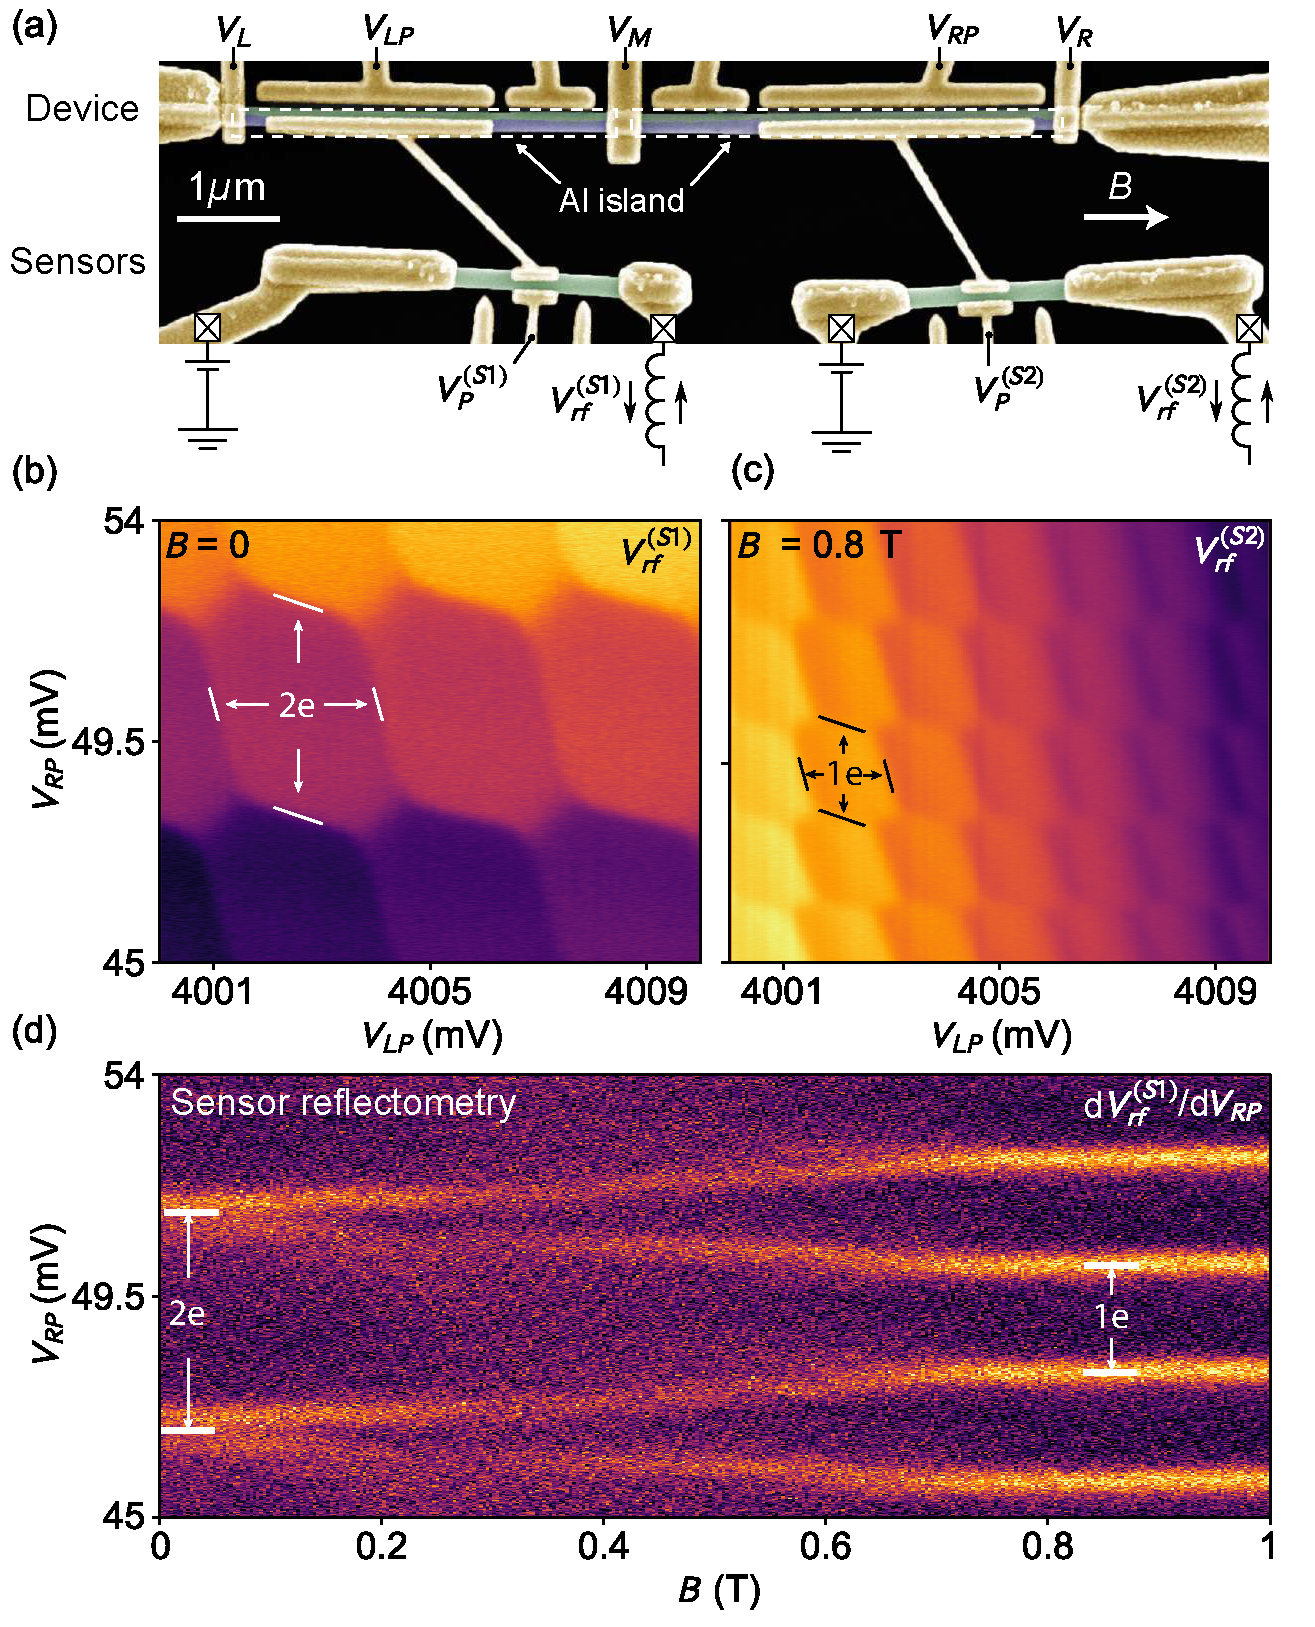
\includegraphics[width=0.7\textwidth]{Fig4-21.pdf}
	\caption[RF charge sensing of double Majorana island]{(a) Scanning electron micrograph of the device (white dashed boxes indicate Al islands). The voltage tunable tunnel barriers are labeled as $V_{L}$, $V_{M}$ and $V_{R}$. Island plunger gates are labeled as $V_{LP}$ and $V_{RP}$ for the left and right island respectively. (b) $2e$-$2e$ periodic superconducting double-island charge stability diagram measured at $B = \SI{0}{\tesla}$ by RF charge sensing with a right sensor. (c) $1e$-$1e$ periodic double-island charge stability diagram measured at $B = \SI{0.8}{\tesla}$ with a left sensor. (d) Charge occupancy of the right island (controlled by $V_{RP}$) evolution as a function of $B$. The color map shows the measured RF demodulated signal from the right sensor ($V^{(S2)}_{rf}$) and is differentiated along the $V_{RP}$ axis. Periodicity change from $2e$ to $1e$ in $V_{RP}$ direction is observed as $B$ is increased.}
	\label{fig:majo_d}
\end{figure}

A double-Majorana-island (white dashed boxes indicate Al islands) device motived by Ref.~\cite{AasenPRX16} is shown in Fig.~\ref{fig:majo_d} (a). Near the main device, two bare InAs NWs, capacitively coupled to each of the islands via floating gates, serve as independent charge sensors of the two islands. Each sensor is part of an independent RF circuit, with $L_{1} = \SI{3.3}{\micro\henry}$ ($f_{\rm res} \sim \SI{60}{\mega\hertz}$) and $L_{2} = \SI{4.7}{\micro\henry}$ ($f_{\rm res} \sim \SI{40}{\mega\hertz}$). Data acquisition used method (3), described above. Gates $V_{L}$, $V_{M}$, and $V_{R}$ were each set to the tunneling regime. Voltages applied to plunger gates $LP$ and $RP$ affect both the carrier density in the semiconductor and the charge offset of each island (see Appendix \ref{sec:majo_D}). Fig.~\ref{fig:majo_d} (b) shows the charge sensing signal of a $2e$-$2e$ periodic superconducting double-island at $B = \SI{0}{\tesla}$, measured using the right charge sensor (S2), with a plane subtracted to remove cross-coupling of the plungers to the three barrier gates, $V_{L}$, $V_{M}$ and $V_{R}$.  Periodic $1e$-$1e$ double-island plane-fitted data, measured using the left charge sensor (S1) at finite magnetic field ($B = \SI{0.8}{\tesla}$) parallel to NW axis, is shown in Fig.~\ref{fig:majo_d} (c). A hexagonal pattern, characteristic of a double-island devices, is readily seen at both zero field and $B = \SI{0.8}{\tesla}$  [Fig.~\ref{fig:majo_d} (b) and Fig.~\ref{fig:majo_d} (c)]. Magnetic field $B$ evolution of the right $2e$ periodic island into the $1e$ periodic island regime, with the left island tuned into a Coulomb valley, is shown in Fig.~\ref{fig:majo_d} (d). The data is differentiated along $V_{RP}$ to improve visibility of the charge transitions.

Previous works \cite{AlbretchNature,sherman} investigated nearly $1e$ periodic island charge occupancy, consistent with an emerging topological phase, using conductance. Using reflectometry and charge instead has  the advantage of not require electron transport through the  device itself. As seen from Fig.~\ref{fig:majo_d} (d), sensing is consistent with these previous transport studies \cite{AlbretchNature}. We will not focus on peak spacing and motion here, to keep the focus on measurement methods.

\subsubsection{Fast charge measurement and signal-to-noise ratios in the \texorpdfstring{$1e$}{1e} regime}

The signal-to-noise ratio (SNR) for detecting the transfer of a single electron between islands of the double-island device in Fig.~\ref{fig:majo_d} (a) was investigated as a function of measurement time using the pulsed gate sequence shown in Fig.~\ref{fig:majo_e} (a). Measurements were done in an applied axial magnetic field $B = \SI{0.6}{\tesla}$, where the charge-stability diagram shows $1e$-$1e$ hexagons. However, in contrast to the tuning in Fig.~\ref{fig:majo_d} (c), $V_{L}$ and $V_{R}$ were set to isolate the double-island, with negligible coupling to the source and drain. Only inter-island transitions [white and red dashed lines in Fig.~\ref{fig:majo_e} (a)] were measurable in this configuration.

A cyclic pulse sequence was applied to gates $LP$ and $RP$ using an arbitrary waveform generator (Tektronix 5014C), placing the system in three configurations, Initialization (I) for \SI{150}{\micro\second}, Preparation (P) for \SI{200}{\micro\second}, and Measurement (M) for a range of times from \SIrange{1}{50}{\micro\second}  [see Fig.~\ref{fig:majo_e} (a) inset and Appendix \ref{sec:majo_C} for details]. The preparation position and duration were chosen to yield roughly equal populations of relaxed and exited populations, which also depended sensitively on the inter-island barrier gate voltage, $V_{M}$. Results of the measurement, integrated over the measurement time, were then binned to form histograms showing the distinguishability of $N$ and $N+2$ charge-difference states ($N = N_{L} - N_{R}$ is the charge difference, where $N_{L}$ and $N_{R}$ are the occupancies of the left and right islands). Note that the number of cycles used to gather histogram statistics does not affect the distinguishability of the two states. More cycles yield a convergence of the histogram to a stable, smooth bimodal distribution. On the other hand, distinguishability of the two populations is affected by the duration at the measurement (M) point. We note that only during the measurement point ($M$) readout was done by triggering the waveform digitizer card [see Appendix \ref{sec:majo_C} for details].

\begin{figure}
	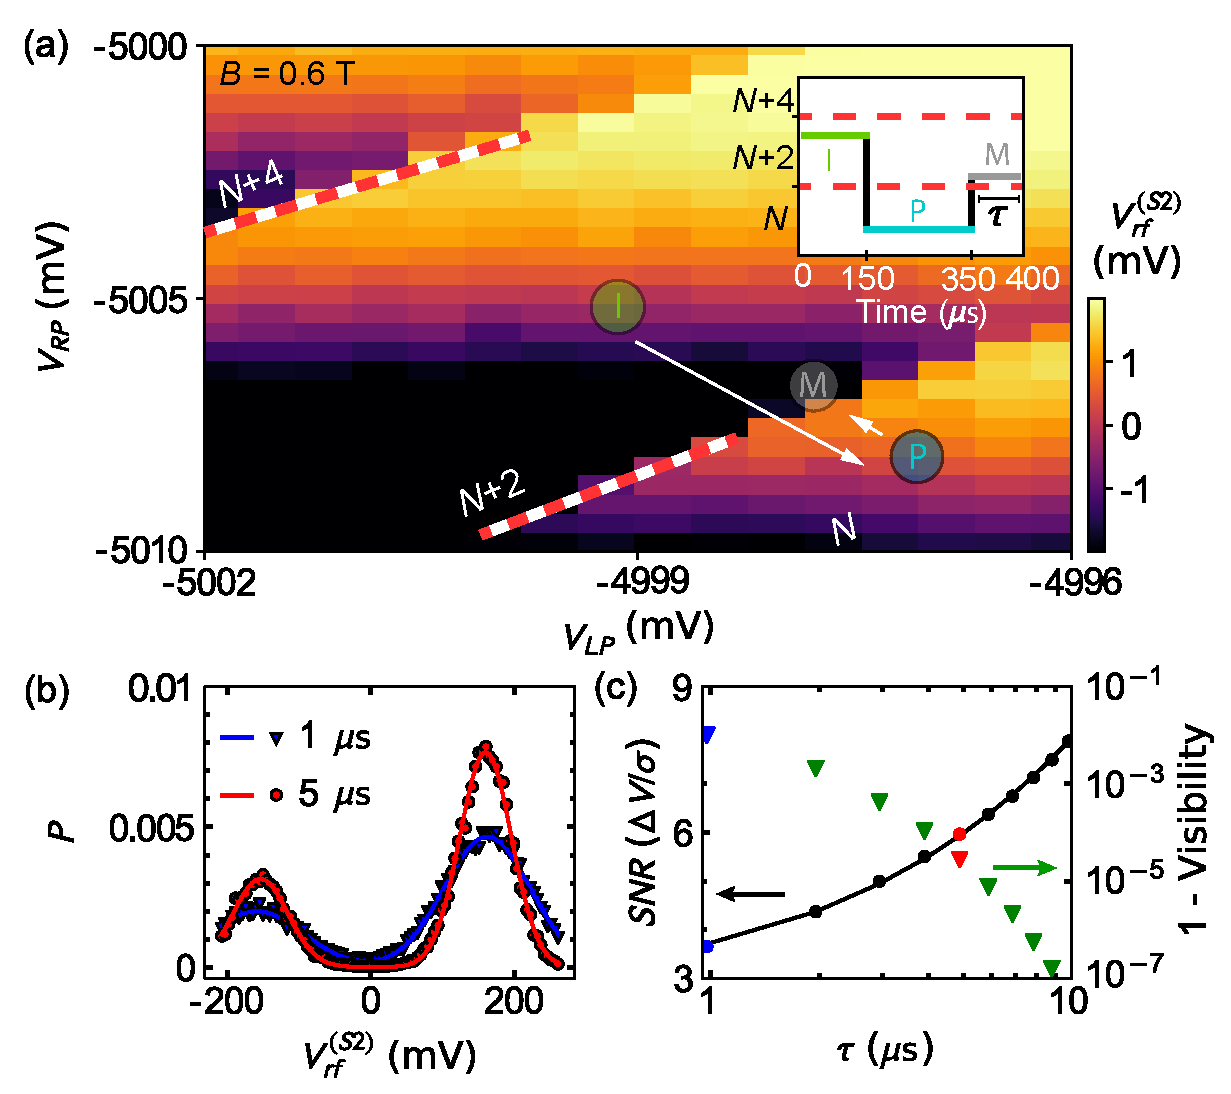
\includegraphics[width=0.65\textwidth]{Fig5-44.pdf}
	\caption[Charge sensitivity and signal-to-noise ratio]{(a) $1e$-$1e$ periodic double-island charge stability diagram at $B = \SI{0.6}{\tesla}$ measured using the right proximal charge sensor. The main device was configured such that tunneling to the left/right lead reservoirs is negligible. Only the inter-island transitions are visible with red and white dashed lines. The relative charge occupancy of the islands is marked as $N$, $N+2$ and $N+4$. The pulse sequence used to characterize signal-to-noise ratio is shown in the inset (see main text and Appendix \ref{sec:majo_C} for description), with positions I, M and P indicated on the charge stability diagram that pulsed gates $LP$ and $RP$ move the system to different gate space positions for a given amount of time. (b) Probability of single shot readout outcomes, $P$, of demodulated voltage signal $V^{(S2)}_{rf}$ for two different measurement times: $\tau = \SI{1}{\micro\second}$ (blue) and $\tau = \SI{5}{\micro\second}$ (red), at the measurement point (M) showing a bimodal relative charge state distribution. c) Signal-to-noise ratio (left axis) at the measurement point (M) together with theory fit. Extracted visibility (right axis) from the double gaussian fits (see main text) as a function of measurement time.}
	\label{fig:majo_e}
\end{figure}

The resulting histogram after $10^{8}$ cycles was fit with a sum of two gaussians,

\begin{equation}
\label{eq:gaussians}
P(V_\textrm{rf}^{(S2)} = A_{N}\exp\left(-\frac{\left(V_{\rm rf}^{(S2)}-\mu_{N}\right)^{2}}{2\sigma_{N}^{2}}\right)
						+ A_{N+2}\exp\left(\frac{-\left(V_{\rm rf}^{(S2)}-\mu_{N+2}\right)^{2}}{2\sigma_{N+2}^{2}}\right)
\end{equation}

where $A$, $\mu$, $\sigma$ are the amplitudes, means, and standard deviations of the $N$ and $N+2$ charge differences. Measured distributions and best fits to Eq.~\eqref{eq:gaussians} for measurement times $\tau = \SI{1}{\micro\second}$ and $\tau = \SI{5}{\micro\second}$ are shown in the Fig.~\ref{fig:majo_e} (b). Separation of the two peaks, $\Delta V$, reflects the sensitivity of the charge sensor, while peak widths $\sigma_{N}$ and $\sigma_{N+2}$ result from measurement noise. We define:
\begin{align}
	\textrm{SNR} = \frac{\Delta V}{\sigma} && (\textrm{where }\sigma^{2} = \sigma_{N}^2+\sigma_{N+2}^2)
\end{align}
Note that Eq.~\eqref{eq:gaussians} does not include relaxation from $N$ to $N+2$ during the measurement. A more complicated form that includes relaxation during measurement was investigated in Ref.~\cite{barthel2009rapid}. In the present case, where $\tau$ is much shorter than the charge relaxation time, as set by $V_{M}$, Eq.~\eqref{eq:gaussians} is valid. The measured SNR as a function of measurement time $\tau$ is shown on the left axis of Fig.~\ref{fig:majo_e} (c). An $\textrm{SNR} > 3$ with an integration time of \SI{1}{\micro\second} was achieved.

Fig.~\ref{fig:majo_e} (c) shows that SNR increased with measurement time, $\tau$, as expected. The simplest model of this dependence, assuming uncorrelated noise \cite{sensingdot}, is:
\begin{equation}
	\textrm{SNR}(\tau) = \frac{\Delta V}{\sigma(\SI{1}{\micro\second})}\left(\frac{\tau+\tau_{0}}{\SI{1}{\micro\second}}\right)^{1/2}
\end{equation}
By using fit parameter $\Delta V = \SI{175.3}{\milli\volt}$, $\tau_{0} = \SI{1.5}{\micro\second}$ and $\sigma(\SI{1}{\micro\second}) = \SI{74.8}{\milli\volt}$, the model yields the curve shown in Fig.~\ref{fig:majo_e} (c), which compares well with the experimentally measured $\textrm{SNR}(\tau)$ in the range \SIrange{1}{10}{\micro\second}. Another quantity that characterizes the quality of detection is the visibility, $V$, defined as the probability of correctly identifying excited and ground states ($N$ and $N+2$) and is expressed as $V = F_{N} + F_{N+2} - 1$, where $F_{N}$ and $F_{N+2}$ are the fidelities calculated following \cite{barthel2009rapid} (see Appendix \ref{sec:majo_C} for details). The resulting dependence of visibility on measurement time, $V(\tau)$, is shown in Fig.~\ref{fig:majo_e} (c), where again effect of relaxation during measurement are neglected. We find $\sigma(\SI{1}{\micro\second}) = 0.998$. These results are comparable to previously reported charge detection studies \cite{PhysRevApplied.11.044061,spin6,sens2,sens3,rf_nw2}.

\subsection{Conclusions}

In summary, we have investigated RF charge sensing and readout of various InAs/Al nanowire devices relevant for Majorana qubits. Charge sensing via a second nanowire capacitively coupled via floating gate to the device allowed charge occupancy in the device to read-out non-invasively and even when visible transport is suppressed through the device. As an application, we followed the evolution of Coulomb charging from $2e$ periodicity to $1e$ periodicity as an axial magnetic field was increased from 0 to 0.6 T, complementing previous conductance measurement of Majorana signatures, without needing to run current through the device. Sensor quality as a function of measurement time was investigated using a pulse sequence that cycled the charge occupancies of the islands. Signal to noise ratio exceeding 3 can be achieved for integration times of \SI{1}{\micro\second} with visibility $V = 99.8\%$. Presented results show that rf resonant circuits coupled to proximal capacitive sensors can be used for fast and detailed characterization.

\subsubsection{Acknowledgments}

We thank Shivendra Upadhyay for help with fabrication, and Wolfgang Pfaff and David Reilly for valuable discussion. Research is supported by Microsoft, the Danish National Research Foundation and by the Australian Research Council Centre of Excellence for Engineered Quantum Systems (project ID CE170100009). PK acknowledges support from ERC starting grant no.~716655. CMM acknowledges support from the Villum Foundation.

